
%(BEGIN_QUESTION)
% Copyright 2014, Tony R. Kuphaldt, released under the Creative Commons Attribution License (v 1.0)
% This means you may do almost anything with this work of mine, so long as you give me proper credit

Use Kirchhoff's Current Law to calculate the magnitudes and directions of currents through {\it all} resistors in this circuit:

$$\includegraphics[width=15.5cm]{i01162x01.eps}$$

\vfil 

\underbar{file i01162}
\eject
%(END_QUESTION)





%(BEGIN_ANSWER)

This is a graded question -- no answers or hints given!

%(END_ANSWER)





%(BEGIN_NOTES)

It is not necessary to know anything about series-parallel or even parallel circuits in order to solve the $R_4$'s current -- all one needs to know is how to use Kirchhoff's Current Law:

$$\includegraphics[width=15.5cm]{i01162x02.eps}$$

%INDEX% Electronics review: series-parallel circuits

%(END_NOTES)


